% Options for packages loaded elsewhere
\PassOptionsToPackage{unicode}{hyperref}
\PassOptionsToPackage{hyphens}{url}
\PassOptionsToPackage{dvipsnames,svgnames,x11names}{xcolor}
%
\documentclass[
  letterpaper,
  DIV=11,
  numbers=noendperiod]{scrartcl}

\usepackage{amsmath,amssymb}
\usepackage{iftex}
\ifPDFTeX
  \usepackage[T1]{fontenc}
  \usepackage[utf8]{inputenc}
  \usepackage{textcomp} % provide euro and other symbols
\else % if luatex or xetex
  \usepackage{unicode-math}
  \defaultfontfeatures{Scale=MatchLowercase}
  \defaultfontfeatures[\rmfamily]{Ligatures=TeX,Scale=1}
\fi
\usepackage{lmodern}
\ifPDFTeX\else  
    % xetex/luatex font selection
\fi
% Use upquote if available, for straight quotes in verbatim environments
\IfFileExists{upquote.sty}{\usepackage{upquote}}{}
\IfFileExists{microtype.sty}{% use microtype if available
  \usepackage[]{microtype}
  \UseMicrotypeSet[protrusion]{basicmath} % disable protrusion for tt fonts
}{}
\makeatletter
\@ifundefined{KOMAClassName}{% if non-KOMA class
  \IfFileExists{parskip.sty}{%
    \usepackage{parskip}
  }{% else
    \setlength{\parindent}{0pt}
    \setlength{\parskip}{6pt plus 2pt minus 1pt}}
}{% if KOMA class
  \KOMAoptions{parskip=half}}
\makeatother
\usepackage{xcolor}
\setlength{\emergencystretch}{3em} % prevent overfull lines
\setcounter{secnumdepth}{-\maxdimen} % remove section numbering
% Make \paragraph and \subparagraph free-standing
\makeatletter
\ifx\paragraph\undefined\else
  \let\oldparagraph\paragraph
  \renewcommand{\paragraph}{
    \@ifstar
      \xxxParagraphStar
      \xxxParagraphNoStar
  }
  \newcommand{\xxxParagraphStar}[1]{\oldparagraph*{#1}\mbox{}}
  \newcommand{\xxxParagraphNoStar}[1]{\oldparagraph{#1}\mbox{}}
\fi
\ifx\subparagraph\undefined\else
  \let\oldsubparagraph\subparagraph
  \renewcommand{\subparagraph}{
    \@ifstar
      \xxxSubParagraphStar
      \xxxSubParagraphNoStar
  }
  \newcommand{\xxxSubParagraphStar}[1]{\oldsubparagraph*{#1}\mbox{}}
  \newcommand{\xxxSubParagraphNoStar}[1]{\oldsubparagraph{#1}\mbox{}}
\fi
\makeatother

\usepackage{color}
\usepackage{fancyvrb}
\newcommand{\VerbBar}{|}
\newcommand{\VERB}{\Verb[commandchars=\\\{\}]}
\DefineVerbatimEnvironment{Highlighting}{Verbatim}{commandchars=\\\{\}}
% Add ',fontsize=\small' for more characters per line
\usepackage{framed}
\definecolor{shadecolor}{RGB}{241,243,245}
\newenvironment{Shaded}{\begin{snugshade}}{\end{snugshade}}
\newcommand{\AlertTok}[1]{\textcolor[rgb]{0.68,0.00,0.00}{#1}}
\newcommand{\AnnotationTok}[1]{\textcolor[rgb]{0.37,0.37,0.37}{#1}}
\newcommand{\AttributeTok}[1]{\textcolor[rgb]{0.40,0.45,0.13}{#1}}
\newcommand{\BaseNTok}[1]{\textcolor[rgb]{0.68,0.00,0.00}{#1}}
\newcommand{\BuiltInTok}[1]{\textcolor[rgb]{0.00,0.23,0.31}{#1}}
\newcommand{\CharTok}[1]{\textcolor[rgb]{0.13,0.47,0.30}{#1}}
\newcommand{\CommentTok}[1]{\textcolor[rgb]{0.37,0.37,0.37}{#1}}
\newcommand{\CommentVarTok}[1]{\textcolor[rgb]{0.37,0.37,0.37}{\textit{#1}}}
\newcommand{\ConstantTok}[1]{\textcolor[rgb]{0.56,0.35,0.01}{#1}}
\newcommand{\ControlFlowTok}[1]{\textcolor[rgb]{0.00,0.23,0.31}{\textbf{#1}}}
\newcommand{\DataTypeTok}[1]{\textcolor[rgb]{0.68,0.00,0.00}{#1}}
\newcommand{\DecValTok}[1]{\textcolor[rgb]{0.68,0.00,0.00}{#1}}
\newcommand{\DocumentationTok}[1]{\textcolor[rgb]{0.37,0.37,0.37}{\textit{#1}}}
\newcommand{\ErrorTok}[1]{\textcolor[rgb]{0.68,0.00,0.00}{#1}}
\newcommand{\ExtensionTok}[1]{\textcolor[rgb]{0.00,0.23,0.31}{#1}}
\newcommand{\FloatTok}[1]{\textcolor[rgb]{0.68,0.00,0.00}{#1}}
\newcommand{\FunctionTok}[1]{\textcolor[rgb]{0.28,0.35,0.67}{#1}}
\newcommand{\ImportTok}[1]{\textcolor[rgb]{0.00,0.46,0.62}{#1}}
\newcommand{\InformationTok}[1]{\textcolor[rgb]{0.37,0.37,0.37}{#1}}
\newcommand{\KeywordTok}[1]{\textcolor[rgb]{0.00,0.23,0.31}{\textbf{#1}}}
\newcommand{\NormalTok}[1]{\textcolor[rgb]{0.00,0.23,0.31}{#1}}
\newcommand{\OperatorTok}[1]{\textcolor[rgb]{0.37,0.37,0.37}{#1}}
\newcommand{\OtherTok}[1]{\textcolor[rgb]{0.00,0.23,0.31}{#1}}
\newcommand{\PreprocessorTok}[1]{\textcolor[rgb]{0.68,0.00,0.00}{#1}}
\newcommand{\RegionMarkerTok}[1]{\textcolor[rgb]{0.00,0.23,0.31}{#1}}
\newcommand{\SpecialCharTok}[1]{\textcolor[rgb]{0.37,0.37,0.37}{#1}}
\newcommand{\SpecialStringTok}[1]{\textcolor[rgb]{0.13,0.47,0.30}{#1}}
\newcommand{\StringTok}[1]{\textcolor[rgb]{0.13,0.47,0.30}{#1}}
\newcommand{\VariableTok}[1]{\textcolor[rgb]{0.07,0.07,0.07}{#1}}
\newcommand{\VerbatimStringTok}[1]{\textcolor[rgb]{0.13,0.47,0.30}{#1}}
\newcommand{\WarningTok}[1]{\textcolor[rgb]{0.37,0.37,0.37}{\textit{#1}}}

\providecommand{\tightlist}{%
  \setlength{\itemsep}{0pt}\setlength{\parskip}{0pt}}\usepackage{longtable,booktabs,array}
\usepackage{calc} % for calculating minipage widths
% Correct order of tables after \paragraph or \subparagraph
\usepackage{etoolbox}
\makeatletter
\patchcmd\longtable{\par}{\if@noskipsec\mbox{}\fi\par}{}{}
\makeatother
% Allow footnotes in longtable head/foot
\IfFileExists{footnotehyper.sty}{\usepackage{footnotehyper}}{\usepackage{footnote}}
\makesavenoteenv{longtable}
\usepackage{graphicx}
\makeatletter
\def\maxwidth{\ifdim\Gin@nat@width>\linewidth\linewidth\else\Gin@nat@width\fi}
\def\maxheight{\ifdim\Gin@nat@height>\textheight\textheight\else\Gin@nat@height\fi}
\makeatother
% Scale images if necessary, so that they will not overflow the page
% margins by default, and it is still possible to overwrite the defaults
% using explicit options in \includegraphics[width, height, ...]{}
\setkeys{Gin}{width=\maxwidth,height=\maxheight,keepaspectratio}
% Set default figure placement to htbp
\makeatletter
\def\fps@figure{htbp}
\makeatother

\KOMAoption{captions}{tableheading}
\makeatletter
\@ifpackageloaded{caption}{}{\usepackage{caption}}
\AtBeginDocument{%
\ifdefined\contentsname
  \renewcommand*\contentsname{Table of contents}
\else
  \newcommand\contentsname{Table of contents}
\fi
\ifdefined\listfigurename
  \renewcommand*\listfigurename{List of Figures}
\else
  \newcommand\listfigurename{List of Figures}
\fi
\ifdefined\listtablename
  \renewcommand*\listtablename{List of Tables}
\else
  \newcommand\listtablename{List of Tables}
\fi
\ifdefined\figurename
  \renewcommand*\figurename{Figure}
\else
  \newcommand\figurename{Figure}
\fi
\ifdefined\tablename
  \renewcommand*\tablename{Table}
\else
  \newcommand\tablename{Table}
\fi
}
\@ifpackageloaded{float}{}{\usepackage{float}}
\floatstyle{ruled}
\@ifundefined{c@chapter}{\newfloat{codelisting}{h}{lop}}{\newfloat{codelisting}{h}{lop}[chapter]}
\floatname{codelisting}{Listing}
\newcommand*\listoflistings{\listof{codelisting}{List of Listings}}
\makeatother
\makeatletter
\makeatother
\makeatletter
\@ifpackageloaded{caption}{}{\usepackage{caption}}
\@ifpackageloaded{subcaption}{}{\usepackage{subcaption}}
\makeatother
\makeatletter
\@ifpackageloaded{tikz}{}{\usepackage{tikz}}
\makeatother
        \newcommand*\circled[1]{\tikz[baseline=(char.base)]{
          \node[shape=circle,draw,inner sep=1pt] (char) {{\scriptsize#1}};}}  
                  

\ifLuaTeX
  \usepackage{selnolig}  % disable illegal ligatures
\fi
\usepackage{bookmark}

\IfFileExists{xurl.sty}{\usepackage{xurl}}{} % add URL line breaks if available
\urlstyle{same} % disable monospaced font for URLs
\hypersetup{
  pdftitle={Week 2: Linear models and causal inference},
  colorlinks=true,
  linkcolor={blue},
  filecolor={Maroon},
  citecolor={Blue},
  urlcolor={Blue},
  pdfcreator={LaTeX via pandoc}}


\title{Week 2: Linear models and causal inference}
\usepackage{etoolbox}
\makeatletter
\providecommand{\subtitle}[1]{% add subtitle to \maketitle
  \apptocmd{\@title}{\par {\large #1 \par}}{}{}
}
\makeatother
\subtitle{Categories and curves}
\author{}
\date{}

\begin{document}
\maketitle


Workspace setup:

\begin{Shaded}
\begin{Highlighting}[]
\FunctionTok{library}\NormalTok{(tidyverse)}
\FunctionTok{library}\NormalTok{(cowplot)}
\FunctionTok{library}\NormalTok{(brms)}
\FunctionTok{library}\NormalTok{(tidybayes)}
\FunctionTok{library}\NormalTok{(patchwork)}
\FunctionTok{library}\NormalTok{(here)}
\end{Highlighting}
\end{Shaded}

As we develop more useful models, we'll begin to practice the art of
generating models with multiple estimands. An \emph{estimand} is a
quantity we want to estimate from the data. Our models may not
themselves produce the answer to our central question, so we need to
know how to calculate these values from the posterior distributions.

This is going to be different from prior regression courses (PSY 612),
where our models were often designed to give us precisely what we
wanted. For example, consider the regression:

\[
\hat{Y} = b_0 + b_1(D)
\] Where \(Y\) is a continuous outcome and \(D\) is a dummy coded
variable (0 = control; 1 = treatment).

\begin{itemize}
\tightlist
\item
  What does \(b_0\) represent?
\item
  What does \(b_1\) represent?
\item
  How would you calculate or estimate the means of both groups from this
  model?
\end{itemize}

\begin{center}\rule{0.5\linewidth}{0.5pt}\end{center}

\subsection{Categories}\label{categories}

If you were to fit the dummy variable model in R, your formula would be:

\begin{verbatim}
y ~ 1 + D
\end{verbatim}

or

\begin{verbatim}
y ~ D # intercept is implied
\end{verbatim}

Forget dummy codes. From here on out, we will incorporate categorical
causes into our models by using index variables. An \textbf{index
variable} contains integers that correspond to different categories. The
numbers have no inherent meaning -- rather, they stand as placeholders
or shorthand for categories.

To fit these models in R, we're going to force the model to drop the
intercept.

\begin{verbatim}
y ~ 0 + I
\end{verbatim}

\begin{center}\rule{0.5\linewidth}{0.5pt}\end{center}

\begin{Shaded}
\begin{Highlighting}[numbers=left,,]
\FunctionTok{data}\NormalTok{(}\StringTok{"Howell1"}\NormalTok{, }\AttributeTok{package =} \StringTok{"rethinking"}\NormalTok{)}
\NormalTok{d }\OtherTok{\textless{}{-}}\NormalTok{ Howell1}
\FunctionTok{library}\NormalTok{(measurements)}
\NormalTok{d}\SpecialCharTok{$}\NormalTok{height }\OtherTok{\textless{}{-}} \FunctionTok{conv\_unit}\NormalTok{(d}\SpecialCharTok{$}\NormalTok{height, }\AttributeTok{from =} \StringTok{"cm"}\NormalTok{, }\AttributeTok{to =} \StringTok{"feet"}\NormalTok{)}
\NormalTok{d}\SpecialCharTok{$}\NormalTok{weight }\OtherTok{\textless{}{-}} \FunctionTok{conv\_unit}\NormalTok{(d}\SpecialCharTok{$}\NormalTok{weight, }\AttributeTok{from =} \StringTok{"kg"}\NormalTok{, }\AttributeTok{to =} \StringTok{"lbs"}\NormalTok{)}
\NormalTok{d }\OtherTok{\textless{}{-}}\NormalTok{ d[d}\SpecialCharTok{$}\NormalTok{age }\SpecialCharTok{\textgreater{}=} \DecValTok{18}\NormalTok{, ]}
\NormalTok{d}\SpecialCharTok{$}\NormalTok{sex }\OtherTok{\textless{}{-}} \FunctionTok{ifelse}\NormalTok{(d}\SpecialCharTok{$}\NormalTok{male }\SpecialCharTok{==} \DecValTok{1}\NormalTok{, }\DecValTok{2}\NormalTok{, }\DecValTok{1}\NormalTok{) }\CommentTok{\# 1 = female, 2 = male}
\NormalTok{d}\SpecialCharTok{$}\NormalTok{sex }\OtherTok{\textless{}{-}} \FunctionTok{factor}\NormalTok{(d}\SpecialCharTok{$}\NormalTok{sex)}
\FunctionTok{head}\NormalTok{(d[, }\FunctionTok{c}\NormalTok{(}\StringTok{"male"}\NormalTok{, }\StringTok{"sex"}\NormalTok{)])}
\end{Highlighting}
\end{Shaded}

\begin{verbatim}
  male sex
1    1   2
2    0   1
3    0   1
4    1   2
5    0   1
6    1   2
\end{verbatim}

\begin{center}\rule{0.5\linewidth}{0.5pt}\end{center}

\subsubsection{Mathematical model}\label{mathematical-model}

Let's write a mathematical model to express weight in terms of sex.

\begin{align*}
w_i &\sim \text{Normal}(\mu_i, \sigma) \\
\mu_i &=     \alpha_{SEX[i]} \\
\alpha_j &\sim \text{Normal}(130, 20)\text{ for }j = 1..2 \\
\sigma &\sim \text{Uniform}(0, 25)
\end{align*}

\subsubsection{\texorpdfstring{Fitting the model using
\texttt{brms()}}{Fitting the model using brms()}}\label{fitting-the-model-using-brms}

\phantomsection\label{annotated-cell-6}%
\begin{Shaded}
\begin{Highlighting}[]
\NormalTok{m1 }\OtherTok{\textless{}{-}} \FunctionTok{brm}\NormalTok{(}
  \AttributeTok{data =}\NormalTok{ d,}
  \AttributeTok{family =}\NormalTok{ gaussian,}
  \FunctionTok{bf}\NormalTok{(weight }\SpecialCharTok{\textasciitilde{}} \DecValTok{0} \SpecialCharTok{+}\NormalTok{ a, }\hspace*{\fill}\NormalTok{\circled{1}}
\NormalTok{     a }\SpecialCharTok{\textasciitilde{}} \DecValTok{0} \SpecialCharTok{+}\NormalTok{ sex, }\hspace*{\fill}\NormalTok{\circled{2}}
     \AttributeTok{nl =} \ConstantTok{TRUE}\NormalTok{), }\hspace*{\fill}\NormalTok{\circled{3}}
  \AttributeTok{prior =} \FunctionTok{c}\NormalTok{(}\FunctionTok{prior}\NormalTok{( }\FunctionTok{normal}\NormalTok{(}\DecValTok{130}\NormalTok{, }\DecValTok{20}\NormalTok{), }\AttributeTok{class=}\NormalTok{b, }\AttributeTok{nlpar =}\NormalTok{ a), }\hspace*{\fill}\NormalTok{\circled{4}}
            \FunctionTok{prior}\NormalTok{( }\FunctionTok{uniform}\NormalTok{(}\DecValTok{0}\NormalTok{, }\DecValTok{25}\NormalTok{),  }\AttributeTok{class=}\NormalTok{sigma, }\AttributeTok{ub=}\DecValTok{25}\NormalTok{)),}
  \AttributeTok{iter =} \DecValTok{2000}\NormalTok{, }\AttributeTok{warmup =} \DecValTok{1000}\NormalTok{, }\AttributeTok{seed =} \DecValTok{3}\NormalTok{, }\AttributeTok{chains=}\DecValTok{1}\NormalTok{,}
  \AttributeTok{file =} \FunctionTok{here}\NormalTok{(}\StringTok{"files/models/22.1"}\NormalTok{)}
\NormalTok{)}
\end{Highlighting}
\end{Shaded}

\begin{description}
\tightlist
\item[\circled{1}]
A few things to note: first is that we've wrapped our formula in the
function \texttt{bf()}, which allows us to build a model with multiple
formulas. Cool. Next, we've forced the model to drop the intercept by
using 0 instead of 1. Finally, we've created a parameter \texttt{a}
which is a constant, but we're going to write another formula to
determine \texttt{a} in the next line. By the way, you can call this
anything you want. Try using \texttt{mean} or anything that will make
sense to you. Just make sure you replace \texttt{a} everywhere else in
the code.
\item[\circled{2}]
Defining \texttt{a}. Again, we drop the intercept, and now \texttt{a} is
determined by the index variable or group.\\
\item[\circled{3}]
This simply allows us to use non-linear language to fit our models, even
though this is a linear model.
\item[\circled{4}]
Once you put yourself in non-linear land, you have to specify which
parameter each prior is for.
\end{description}

\begin{center}\rule{0.5\linewidth}{0.5pt}\end{center}

\begin{Shaded}
\begin{Highlighting}[]
\FunctionTok{posterior\_summary}\NormalTok{(m1)}
\end{Highlighting}
\end{Shaded}

\begin{verbatim}
            Estimate  Est.Error        Q2.5       Q97.5
b_a_sex1    92.27947 0.91187785    90.50115    94.05188
b_a_sex2   107.22803 0.91554891   105.57421   109.04851
sigma       12.19829 0.46172983    11.34413    13.13513
lprior     -13.47705 0.09932469   -13.66427   -13.27516
lp__     -1390.30623 1.23903576 -1393.80224 -1388.90647
\end{verbatim}

Here, we are given the estimates of the parameters specified in our
model: the average weight of women (\texttt{b\_a\_sex1}) and the average
weight of men (\texttt{b\_a\_sex2}). But our question is whether these
average weights are different. How do we get that?

\begin{center}\rule{0.5\linewidth}{0.5pt}\end{center}

\begin{Shaded}
\begin{Highlighting}[]
\NormalTok{post }\OtherTok{=} \FunctionTok{as\_draws\_df}\NormalTok{(m1) }
\FunctionTok{head}\NormalTok{(post)}
\end{Highlighting}
\end{Shaded}

\begin{verbatim}
# A draws_df: 6 iterations, 1 chains, and 5 variables
  b_a_sex1 b_a_sex2 sigma lprior  lp__
1       92      106    13    -14 -1391
2       92      109    13    -13 -1391
3       91      109    12    -13 -1392
4       92      109    12    -13 -1391
5       92      109    12    -13 -1391
6       91      106    13    -14 -1391
# ... hidden reserved variables {'.chain', '.iteration', '.draw'}
\end{verbatim}

\begin{Shaded}
\begin{Highlighting}[]
\NormalTok{post }\SpecialCharTok{\%\textgreater{}\%} 
  \FunctionTok{mutate}\NormalTok{(}\AttributeTok{diff\_fm =}\NormalTok{ b\_a\_sex1 }\SpecialCharTok{{-}}\NormalTok{ b\_a\_sex2) }\SpecialCharTok{\%\textgreater{}\%} 
  \FunctionTok{pivot\_longer}\NormalTok{(}\AttributeTok{cols =} \FunctionTok{c}\NormalTok{(b\_a\_sex1}\SpecialCharTok{:}\NormalTok{sigma, diff\_fm)) }\SpecialCharTok{\%\textgreater{}\%} 
  \FunctionTok{group\_by}\NormalTok{(name) }\SpecialCharTok{\%\textgreater{}\%} 
  \FunctionTok{mean\_qi}\NormalTok{(value, }\AttributeTok{.width =}\NormalTok{ .}\DecValTok{89}\NormalTok{)}
\end{Highlighting}
\end{Shaded}

\begin{verbatim}
Warning: Dropping 'draws_df' class as required metadata was removed.
\end{verbatim}

\begin{verbatim}
# A tibble: 4 x 7
  name     value .lower .upper .width .point .interval
  <chr>    <dbl>  <dbl>  <dbl>  <dbl> <chr>  <chr>    
1 b_a_sex1  92.3   90.9   93.8   0.89 mean   qi       
2 b_a_sex2 107.   106.   109.    0.89 mean   qi       
3 diff_fm  -14.9  -17.0  -12.9   0.89 mean   qi       
4 sigma     12.2   11.5   12.9   0.89 mean   qi       
\end{verbatim}

\begin{center}\rule{0.5\linewidth}{0.5pt}\end{center}

\subsubsection{Calculate the contrast}\label{calculate-the-contrast}

We can create two plots. One is the posterior distributions of average
female and male weights and one is the average difference.

\begin{Shaded}
\begin{Highlighting}[]
\NormalTok{p1 }\OtherTok{\textless{}{-}}\NormalTok{ post }\SpecialCharTok{\%\textgreater{}\%} 
  \FunctionTok{pivot\_longer}\NormalTok{(}\FunctionTok{starts\_with}\NormalTok{(}\StringTok{"b"}\NormalTok{)) }\SpecialCharTok{\%\textgreater{}\%} 
  \FunctionTok{mutate}\NormalTok{(}\AttributeTok{sex =} \FunctionTok{ifelse}\NormalTok{(}\FunctionTok{str\_detect}\NormalTok{(name, }\StringTok{"1"}\NormalTok{), }\StringTok{"female"}\NormalTok{, }\StringTok{"male"}\NormalTok{)) }\SpecialCharTok{\%\textgreater{}\%} 
  \FunctionTok{ggplot}\NormalTok{(}\FunctionTok{aes}\NormalTok{(}\AttributeTok{x=}\NormalTok{value, }\AttributeTok{color =}\NormalTok{ sex)) }\SpecialCharTok{+}
  \FunctionTok{geom\_density}\NormalTok{(}\AttributeTok{linewidth =} \DecValTok{2}\NormalTok{) }\SpecialCharTok{+}
  \FunctionTok{labs}\NormalTok{(}\AttributeTok{x =} \StringTok{"weight(lbs)"}\NormalTok{) }

\NormalTok{p2 }\OtherTok{\textless{}{-}}\NormalTok{ post }\SpecialCharTok{\%\textgreater{}\%} 
  \FunctionTok{mutate}\NormalTok{(}\AttributeTok{diff\_fm =}\NormalTok{ b\_a\_sex1 }\SpecialCharTok{{-}}\NormalTok{ b\_a\_sex2) }\SpecialCharTok{\%\textgreater{}\%}
  \FunctionTok{ggplot}\NormalTok{(}\FunctionTok{aes}\NormalTok{(}\AttributeTok{x=}\NormalTok{diff\_fm)) }\SpecialCharTok{+}
  \FunctionTok{geom\_density}\NormalTok{(}\AttributeTok{linewidth =} \DecValTok{2}\NormalTok{) }\SpecialCharTok{+}
  \FunctionTok{labs}\NormalTok{(}\AttributeTok{x =} \StringTok{"difference in weight(lbs)"}\NormalTok{) }

\NormalTok{( p1 }\SpecialCharTok{|}\NormalTok{ p2)}
\end{Highlighting}
\end{Shaded}

\begin{center}\rule{0.5\linewidth}{0.5pt}\end{center}

\begin{verbatim}
Warning: Dropping 'draws_df' class as required metadata was removed.
\end{verbatim}

\begin{center}
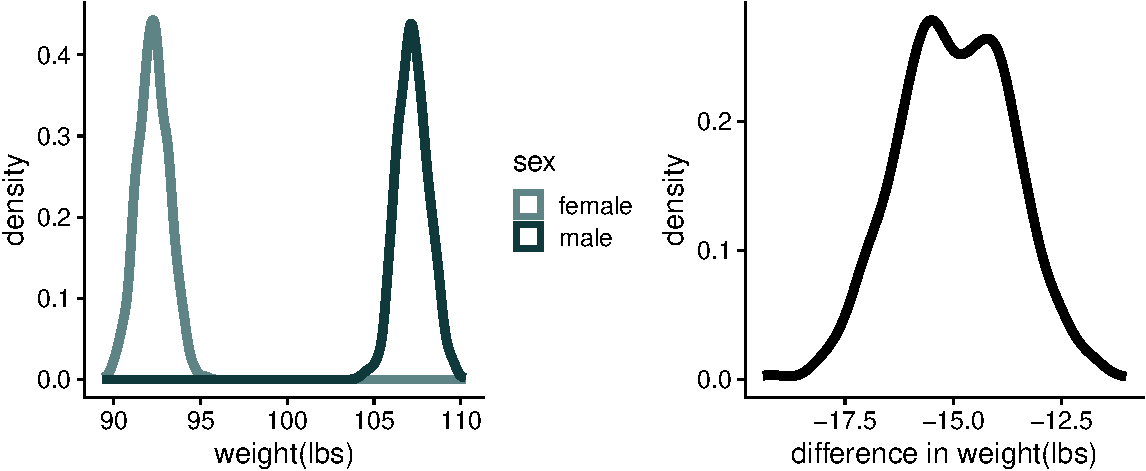
\includegraphics[width=25in,height=\textheight]{lecture02-2_files/figure-pdf/unnamed-chunk-7-1.pdf}
\end{center}

\begin{center}\rule{0.5\linewidth}{0.5pt}\end{center}

\subsubsection{Expected values vs predicted
values}\label{expected-values-vs-predicted-values}

A note that the distributions of the \emph{mean} weights is not the same
as the distribution of weights period. For that, we need the posterior
predictive distributions. Here are two methods for getting predicted
values.

\textbf{Method 1:} simulate using the \texttt{rnorm()}function. This is
more intuitive and will help you mentally reconnect the parameters of
your statistical model with the causal model you started with. But
there's more room for human error.

\begin{Shaded}
\begin{Highlighting}[]
\NormalTok{pred\_f  }\OtherTok{\textless{}{-}} \FunctionTok{rnorm}\NormalTok{(}\FunctionTok{nrow}\NormalTok{(post), }\AttributeTok{mean =}\NormalTok{ post}\SpecialCharTok{$}\NormalTok{b\_a\_sex1, }\AttributeTok{sd =}\NormalTok{ post}\SpecialCharTok{$}\NormalTok{sigma )}
\NormalTok{pred\_m  }\OtherTok{\textless{}{-}} \FunctionTok{rnorm}\NormalTok{(}\FunctionTok{nrow}\NormalTok{(post), }\AttributeTok{mean =}\NormalTok{ post}\SpecialCharTok{$}\NormalTok{b\_a\_sex2, }\AttributeTok{sd =}\NormalTok{ post}\SpecialCharTok{$}\NormalTok{sigma )}

\NormalTok{pred\_post }\OtherTok{=} \FunctionTok{data.frame}\NormalTok{(pred\_f, pred\_m) }\SpecialCharTok{\%\textgreater{}\%}
  \FunctionTok{mutate}\NormalTok{(}\AttributeTok{diff =}\NormalTok{ pred\_f}\SpecialCharTok{{-}}\NormalTok{pred\_m)}
\FunctionTok{head}\NormalTok{(pred\_post)}
\end{Highlighting}
\end{Shaded}

\begin{verbatim}
     pred_f    pred_m       diff
1  86.32946 116.12303 -29.793568
2 118.30647 112.73086   5.575613
3 117.37189 109.49416   7.877728
4  84.66887 118.14646 -33.477588
5  71.35264 139.37554 -68.022901
6  69.13076  94.41733 -25.286567
\end{verbatim}

\begin{center}\rule{0.5\linewidth}{0.5pt}\end{center}

\subsubsection{Expected values vs predicted
values}\label{expected-values-vs-predicted-values-1}

\textbf{Method 2:} use the \texttt{predicted\_draws()} function. This is
less intuitive, but there's less room for you to make a mistake.

\begin{Shaded}
\begin{Highlighting}[]
\NormalTok{nd }\OtherTok{=} \FunctionTok{distinct}\NormalTok{(d, sex)}
\NormalTok{pred\_all }\OtherTok{=} \FunctionTok{predicted\_draws}\NormalTok{(}\AttributeTok{object=}\NormalTok{m1, }\AttributeTok{newdata=}\NormalTok{nd) }\SpecialCharTok{\%\textgreater{}\%} 
\NormalTok{  ungroup }\SpecialCharTok{\%\textgreater{}\%} \FunctionTok{select}\NormalTok{(}\SpecialCharTok{{-}}\NormalTok{.row) }\SpecialCharTok{\%\textgreater{}\%} 
  \FunctionTok{pivot\_wider}\NormalTok{(}\AttributeTok{names\_from =}\NormalTok{ sex, }\AttributeTok{names\_prefix =} \StringTok{"sex"}\NormalTok{, }\AttributeTok{values\_from =}\NormalTok{ .prediction) }\SpecialCharTok{\%\textgreater{}\%} 
  \FunctionTok{mutate}\NormalTok{(}\AttributeTok{diff =}\NormalTok{ sex1}\SpecialCharTok{{-}}\NormalTok{sex2)}
\FunctionTok{head}\NormalTok{(pred\_all)}
\end{Highlighting}
\end{Shaded}

\begin{verbatim}
# A tibble: 6 x 6
  .chain .iteration .draw  sex2  sex1    diff
   <int>      <int> <int> <dbl> <dbl>   <dbl>
1     NA         NA     1 110.   99.0 -11.3  
2     NA         NA     2 110.   75.1 -34.5  
3     NA         NA     3 116.   90.4 -25.6  
4     NA         NA     4  93.5  80.4 -13.1  
5     NA         NA     5 120.   77.1 -42.4  
6     NA         NA     6  98.4  99.4   0.996
\end{verbatim}

\begin{center}\rule{0.5\linewidth}{0.5pt}\end{center}

\begin{Shaded}
\begin{Highlighting}[]
\CommentTok{\# plot male and female distributions using the first version}
\NormalTok{p1 }\OtherTok{\textless{}{-}}\NormalTok{ pred\_post }\SpecialCharTok{\%\textgreater{}\%} \FunctionTok{pivot\_longer}\NormalTok{(}\FunctionTok{starts\_with}\NormalTok{(}\StringTok{"pred"}\NormalTok{)) }\SpecialCharTok{\%\textgreater{}\%} 
  \FunctionTok{mutate}\NormalTok{(}\AttributeTok{sex =} \FunctionTok{ifelse}\NormalTok{(name }\SpecialCharTok{==} \StringTok{"pred\_f"}\NormalTok{, }\StringTok{"female"}\NormalTok{, }\StringTok{"male"}\NormalTok{)) }\SpecialCharTok{\%\textgreater{}\%} 
  \FunctionTok{ggplot}\NormalTok{(}\FunctionTok{aes}\NormalTok{(}\AttributeTok{x =}\NormalTok{ value, }\AttributeTok{color =}\NormalTok{ sex)) }\SpecialCharTok{+}
  \FunctionTok{geom\_density}\NormalTok{(}\AttributeTok{linewidth =} \DecValTok{2}\NormalTok{) }\SpecialCharTok{+}
  \FunctionTok{labs}\NormalTok{(}\AttributeTok{x =} \StringTok{"weight (lbs)"}\NormalTok{)}

\CommentTok{\# plot difference distribution using the second version}
\CommentTok{\# Compute density first}
\NormalTok{density\_data }\OtherTok{\textless{}{-}} \FunctionTok{density}\NormalTok{(pred\_all}\SpecialCharTok{$}\NormalTok{diff)}

\CommentTok{\# Convert to a tibble for plotting}
\NormalTok{density\_df }\OtherTok{\textless{}{-}} \FunctionTok{tibble}\NormalTok{(}
  \AttributeTok{x =}\NormalTok{ density\_data}\SpecialCharTok{$}\NormalTok{x,}
  \AttributeTok{y =}\NormalTok{ density\_data}\SpecialCharTok{$}\NormalTok{y,}
  \AttributeTok{fill\_group =} \FunctionTok{ifelse}\NormalTok{(x }\SpecialCharTok{\textless{}} \DecValTok{0}\NormalTok{, }\StringTok{"male"}\NormalTok{, }\StringTok{"female"}\NormalTok{)  }\CommentTok{\# Define fill condition}
\NormalTok{)}

\CommentTok{\# Plot with area fill}
\NormalTok{p2 }\OtherTok{\textless{}{-}} \FunctionTok{ggplot}\NormalTok{(density\_df, }\FunctionTok{aes}\NormalTok{(}\AttributeTok{x =}\NormalTok{ x, }\AttributeTok{y =}\NormalTok{ y, }\AttributeTok{fill =}\NormalTok{ fill\_group)) }\SpecialCharTok{+}
  \FunctionTok{geom\_area}\NormalTok{() }\SpecialCharTok{+}  \CommentTok{\# Adjust transparency if needed}
  \FunctionTok{geom\_line}\NormalTok{(}\AttributeTok{linewidth =} \FloatTok{1.2}\NormalTok{, }\AttributeTok{color =} \StringTok{"black"}\NormalTok{) }\SpecialCharTok{+}  \CommentTok{\# Keep one continuous curve}
  \FunctionTok{labs}\NormalTok{(}\AttributeTok{x =} \StringTok{"Difference in weight (F{-}M)"}\NormalTok{, }\AttributeTok{y =} \StringTok{"density"}\NormalTok{) }\SpecialCharTok{+}
  \FunctionTok{guides}\NormalTok{(}\AttributeTok{fill =} \StringTok{"none"}\NormalTok{)}

\NormalTok{(p1 }\SpecialCharTok{|}\NormalTok{ p2)}
\end{Highlighting}
\end{Shaded}

\begin{center}
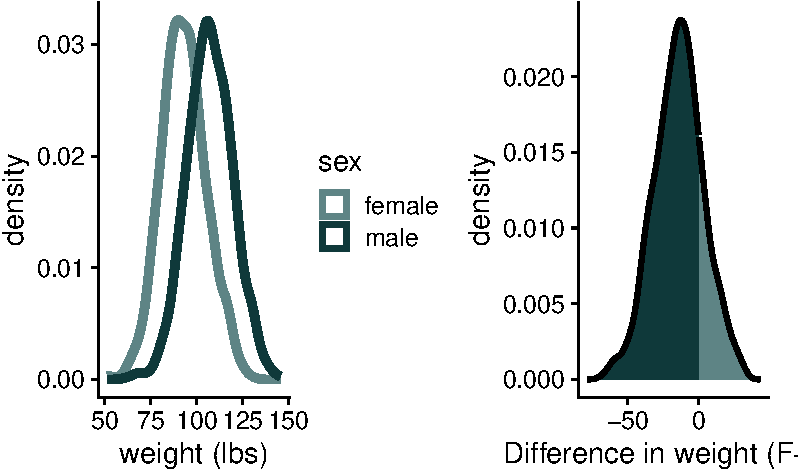
\includegraphics[width=17.1875in,height=\textheight]{lecture02-2_files/figure-pdf/unnamed-chunk-9-1.pdf}
\end{center}

\begin{center}\rule{0.5\linewidth}{0.5pt}\end{center}

\subsection{exercise}\label{exercise}

In the \texttt{rethinking} package, the dataset \texttt{milk} contains
information about the composition of milk across primate species, as
well as some other facts about those species. The taxonomic membership
of each species is included in the variable \texttt{clade}; there are
four categories.

\begin{enumerate}
\def\labelenumi{\arabic{enumi}.}
\tightlist
\item
  Create variable in the dataset to assign an index value to each of the
  4 categories.
\item
  Standardize the milk energy variable (\texttt{kcal.per.g}).
  \footnote{You don't need to be an expert in primate biology to have a
    sense of what is reasonable for these values after we standardize.}
\item
  Write a mathematical model to express the average milk energy (in
  standardized kilocalories) in each clade.
\end{enumerate}

\begin{center}\rule{0.5\linewidth}{0.5pt}\end{center}

\subsubsection{solution}\label{solution}

\begin{Shaded}
\begin{Highlighting}[]
\FunctionTok{data}\NormalTok{(}\StringTok{"milk"}\NormalTok{, }\AttributeTok{package=}\StringTok{"rethinking"}\NormalTok{)}
\FunctionTok{str}\NormalTok{(milk)}
\end{Highlighting}
\end{Shaded}

\begin{verbatim}
'data.frame':   29 obs. of  8 variables:
 $ clade         : Factor w/ 4 levels "Ape","New World Monkey",..: 4 4 4 4 4 2 2 2 2 2 ...
 $ species       : Factor w/ 29 levels "A palliata","Alouatta seniculus",..: 11 8 9 10 16 2 1 6 28 27 ...
 $ kcal.per.g    : num  0.49 0.51 0.46 0.48 0.6 0.47 0.56 0.89 0.91 0.92 ...
 $ perc.fat      : num  16.6 19.3 14.1 14.9 27.3 ...
 $ perc.protein  : num  15.4 16.9 16.9 13.2 19.5 ...
 $ perc.lactose  : num  68 63.8 69 71.9 53.2 ...
 $ mass          : num  1.95 2.09 2.51 1.62 2.19 5.25 5.37 2.51 0.71 0.68 ...
 $ neocortex.perc: num  55.2 NA NA NA NA ...
\end{verbatim}

\begin{Shaded}
\begin{Highlighting}[]
\NormalTok{milk}\SpecialCharTok{$}\NormalTok{clade\_id }\OtherTok{\textless{}{-}} \FunctionTok{as.integer}\NormalTok{(milk}\SpecialCharTok{$}\NormalTok{clade)}
\NormalTok{milk}\SpecialCharTok{$}\NormalTok{clade\_id }\OtherTok{\textless{}{-}} \FunctionTok{as.factor}\NormalTok{(milk}\SpecialCharTok{$}\NormalTok{clade\_id)}
\NormalTok{milk}\SpecialCharTok{$}\NormalTok{K }\OtherTok{\textless{}{-}}\NormalTok{ rethinking}\SpecialCharTok{::}\FunctionTok{standardize}\NormalTok{(milk}\SpecialCharTok{$}\NormalTok{kcal.per.g)}
\end{Highlighting}
\end{Shaded}

\begin{center}\rule{0.5\linewidth}{0.5pt}\end{center}

\begin{align*}
K_i &\sim \text{Normal}(\mu_i, \sigma) \\
\mu_i &= \alpha_{\text{CLADE}[i]} \\
\alpha_i &\sim \text{Normal}(0, 0.5) \text{ for }j=1..4 \\
\sigma &\sim \text{Exponential}(1) \\
\end{align*}

\textbf{Exercise:} Now fit your model using \texttt{brms()}. It's ok if
your mathematical model is a bit different from mine.

\begin{center}\rule{0.5\linewidth}{0.5pt}\end{center}

\subsubsection{solution}\label{solution-1}

\begin{Shaded}
\begin{Highlighting}[]
\NormalTok{m2 }\OtherTok{\textless{}{-}} \FunctionTok{brm}\NormalTok{(}
  \AttributeTok{data=}\NormalTok{milk,}
  \AttributeTok{family=}\NormalTok{gaussian,}
  \FunctionTok{bf}\NormalTok{(K }\SpecialCharTok{\textasciitilde{}} \DecValTok{0} \SpecialCharTok{+}\NormalTok{ a,}
\NormalTok{     a }\SpecialCharTok{\textasciitilde{}} \DecValTok{0} \SpecialCharTok{+}\NormalTok{ clade\_id,}
     \AttributeTok{nl =} \ConstantTok{TRUE}\NormalTok{),}
  \AttributeTok{prior =} \FunctionTok{c}\NormalTok{( }\FunctionTok{prior}\NormalTok{(}\FunctionTok{normal}\NormalTok{(}\DecValTok{0}\NormalTok{,.}\DecValTok{5}\NormalTok{), }\AttributeTok{class=}\NormalTok{b, }\AttributeTok{nlpar=}\NormalTok{a),}
             \FunctionTok{prior}\NormalTok{(}\FunctionTok{exponential}\NormalTok{(}\DecValTok{1}\NormalTok{), }\AttributeTok{class=}\NormalTok{sigma)),}
  \AttributeTok{iter =} \DecValTok{2000}\NormalTok{, }\AttributeTok{warmup =} \DecValTok{1000}\NormalTok{, }\AttributeTok{seed =} \DecValTok{3}\NormalTok{, }\AttributeTok{chains=}\DecValTok{1}\NormalTok{,}
  \AttributeTok{file =} \FunctionTok{here}\NormalTok{(}\StringTok{"files/models/22.2"}\NormalTok{)}
\NormalTok{)}

\FunctionTok{posterior\_summary}\NormalTok{(m2)}
\end{Highlighting}
\end{Shaded}

\begin{verbatim}
                 Estimate Est.Error         Q2.5        Q97.5
b_a_clade_id1  -0.4641202 0.2256089  -0.89176596  -0.03325312
b_a_clade_id2   0.3417955 0.2276394  -0.12749964   0.78516752
b_a_clade_id3   0.6493047 0.2857904   0.09024468   1.18518255
b_a_clade_id4  -0.5387150 0.2962131  -1.10847821   0.03517569
sigma           0.7991983 0.1178092   0.61678499   1.07557053
lprior         -4.3341786 1.1496078  -6.91138553  -2.49326609
lp__          -38.8228118 1.5985564 -42.59133454 -36.64554417
\end{verbatim}

\begin{center}\rule{0.5\linewidth}{0.5pt}\end{center}

\subsubsection{exercise}\label{exercise-1}

Plot the following distributions:

\begin{itemize}
\tightlist
\item
  Posterior distribution of average milk energy by clade.
\item
  Posterior distribution of predicted milk energy values by clade.
\end{itemize}

\begin{center}\rule{0.5\linewidth}{0.5pt}\end{center}

\subsubsection{solution}\label{solution-2}

\begin{Shaded}
\begin{Highlighting}[]
\NormalTok{post }\OtherTok{\textless{}{-}} \FunctionTok{as\_draws\_df}\NormalTok{( m2 )}
\NormalTok{post }\SpecialCharTok{\%\textgreater{}\%} 
  \FunctionTok{pivot\_longer}\NormalTok{(}\FunctionTok{starts\_with}\NormalTok{(}\StringTok{"b"}\NormalTok{)) }\SpecialCharTok{\%\textgreater{}\%} 
  \FunctionTok{mutate}\NormalTok{(}
    \AttributeTok{name =} \FunctionTok{str\_extract}\NormalTok{(name, }\StringTok{"[0{-}9]"}\NormalTok{),}
    \AttributeTok{name =} \FunctionTok{factor}\NormalTok{(name, }\AttributeTok{labels =} \FunctionTok{levels}\NormalTok{(milk}\SpecialCharTok{$}\NormalTok{clade))) }\SpecialCharTok{\%\textgreater{}\%} 
  \FunctionTok{ggplot}\NormalTok{(}\FunctionTok{aes}\NormalTok{(}\AttributeTok{x =}\NormalTok{ value, }\AttributeTok{color =}\NormalTok{ name)) }\SpecialCharTok{+}
  \FunctionTok{geom\_density}\NormalTok{(}\AttributeTok{linewidth =} \DecValTok{2}\NormalTok{) }\SpecialCharTok{+}
  \FunctionTok{labs}\NormalTok{(}\AttributeTok{title =} \StringTok{"Posterior distribution of expected milk energy"}\NormalTok{) }\SpecialCharTok{+}
  \FunctionTok{theme}\NormalTok{(}\AttributeTok{legend.position =} \StringTok{"bottom"}\NormalTok{)}
\end{Highlighting}
\end{Shaded}

\begin{verbatim}
Warning: Dropping 'draws_df' class as required metadata was removed.
\end{verbatim}

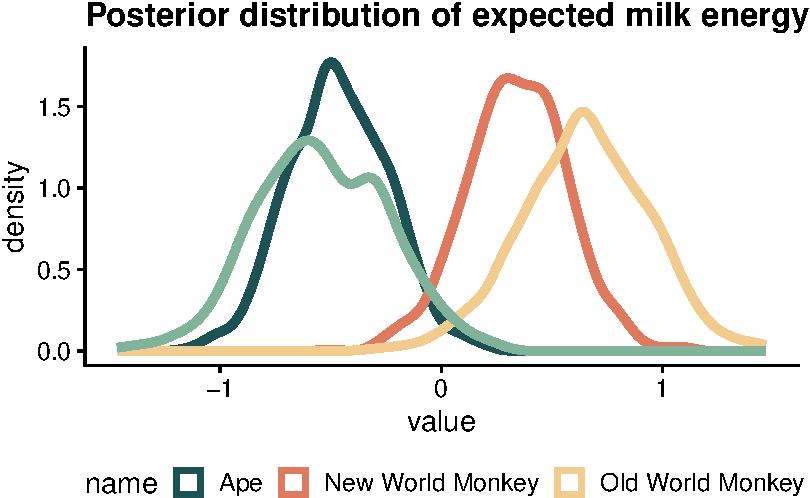
\includegraphics[width=17.1875in,height=\textheight]{lecture02-2_files/figure-pdf/unnamed-chunk-12-1.pdf}

\begin{center}\rule{0.5\linewidth}{0.5pt}\end{center}

\subsubsection{solution}\label{solution-3}

\begin{Shaded}
\begin{Highlighting}[]
\NormalTok{nd }\OtherTok{=} \FunctionTok{distinct}\NormalTok{(milk, clade\_id)}
\NormalTok{ppd }\OtherTok{\textless{}{-}} \FunctionTok{posterior\_predict}\NormalTok{( m2, }\AttributeTok{newdata =}\NormalTok{ nd)}
\NormalTok{ppd }\OtherTok{=} \FunctionTok{as.data.frame}\NormalTok{(ppd)}
\FunctionTok{names}\NormalTok{(ppd) }\OtherTok{=} \FunctionTok{levels}\NormalTok{(milk}\SpecialCharTok{$}\NormalTok{clade)}
\NormalTok{ppd }\SpecialCharTok{\%\textgreater{}\%} 
  \FunctionTok{pivot\_longer}\NormalTok{(}\FunctionTok{everything}\NormalTok{()) }\SpecialCharTok{\%\textgreater{}\%} 
  \FunctionTok{ggplot}\NormalTok{(}\FunctionTok{aes}\NormalTok{(}\AttributeTok{x =}\NormalTok{ value, }\AttributeTok{color =}\NormalTok{ name)) }\SpecialCharTok{+}
  \FunctionTok{geom\_density}\NormalTok{(}\AttributeTok{linewidth =} \DecValTok{2}\NormalTok{) }\SpecialCharTok{+}
  \FunctionTok{labs}\NormalTok{(}\AttributeTok{title =} \StringTok{"Posterior predictive distribution of predicted milk energy"}\NormalTok{) }\SpecialCharTok{+}
  \FunctionTok{theme}\NormalTok{(}\AttributeTok{legend.position =} \StringTok{"bottom"}\NormalTok{)}
\end{Highlighting}
\end{Shaded}

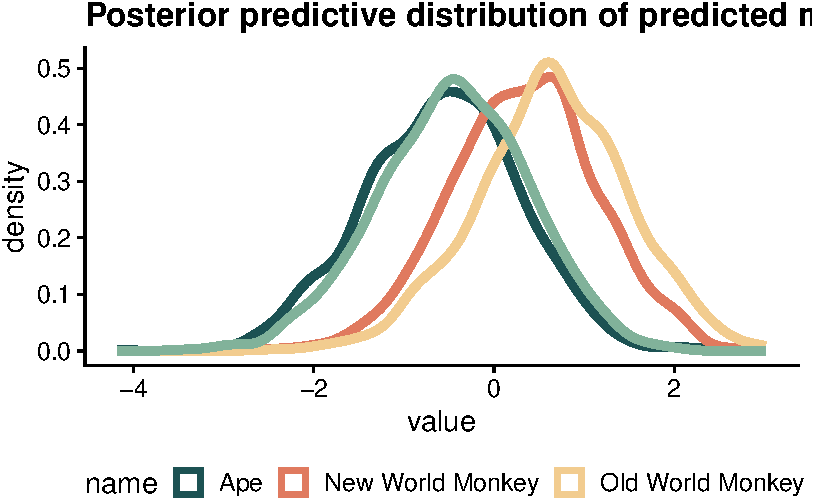
\includegraphics[width=17.1875in,height=\textheight]{lecture02-2_files/figure-pdf/unnamed-chunk-13-1.pdf}

\begin{center}\rule{0.5\linewidth}{0.5pt}\end{center}

\subsubsection{\texorpdfstring{Plotting with \texttt{brms} and
\texttt{tidybayes}}{Plotting with brms and tidybayes}}\label{plotting-with-brms-and-tidybayes}

\begin{Shaded}
\begin{Highlighting}[]
\FunctionTok{as\_draws\_df}\NormalTok{(m2) }\SpecialCharTok{\%\textgreater{}\%} 
  \FunctionTok{pivot\_longer}\NormalTok{(}\FunctionTok{starts\_with}\NormalTok{(}\StringTok{"b"}\NormalTok{)) }\SpecialCharTok{\%\textgreater{}\%} 
  \FunctionTok{mutate}\NormalTok{(}
    \AttributeTok{clade =} \FunctionTok{str\_extract}\NormalTok{(name, }\StringTok{"[0{-}9]"}\NormalTok{),}
    \AttributeTok{clade =} \FunctionTok{as.numeric}\NormalTok{(clade),}
    \AttributeTok{clade =} \FunctionTok{factor}\NormalTok{(clade, }\AttributeTok{labels=}\FunctionTok{levels}\NormalTok{(milk}\SpecialCharTok{$}\NormalTok{clade))}
\NormalTok{  ) }\SpecialCharTok{\%\textgreater{}\%}
  \FunctionTok{ggplot}\NormalTok{(}\FunctionTok{aes}\NormalTok{(}\AttributeTok{y =}\NormalTok{ clade, }\AttributeTok{x =}\NormalTok{ value)) }\SpecialCharTok{+}
  \FunctionTok{stat\_halfeye}\NormalTok{() }\SpecialCharTok{+}
  \FunctionTok{labs}\NormalTok{(}\AttributeTok{x=}\StringTok{"mean"}\NormalTok{, }\AttributeTok{y=}\ConstantTok{NULL}\NormalTok{)}
\end{Highlighting}
\end{Shaded}

\begin{verbatim}
Warning: Dropping 'draws_df' class as required metadata was removed.
\end{verbatim}

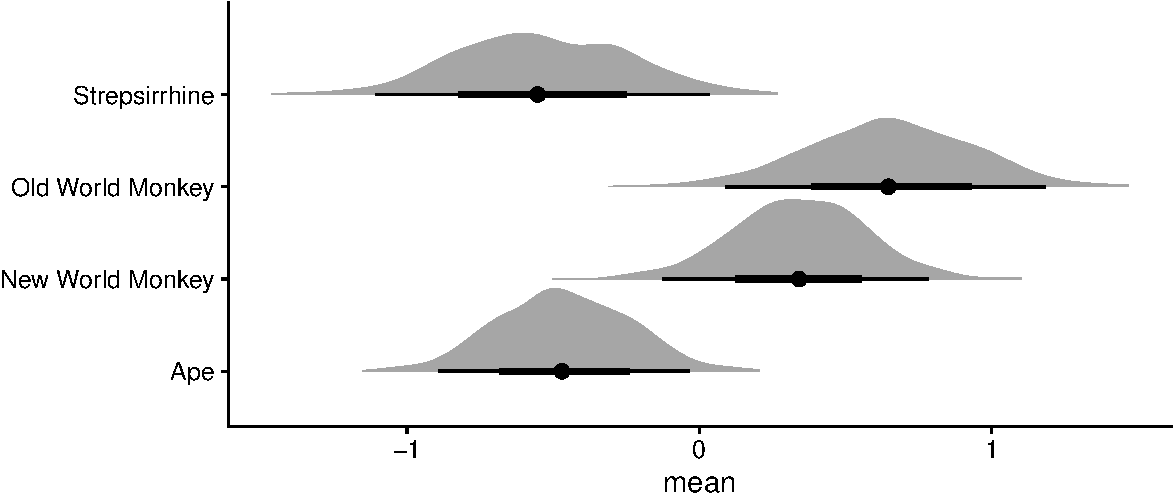
\includegraphics[width=25in,height=\textheight]{lecture02-2_files/figure-pdf/unnamed-chunk-14-1.pdf}

\begin{center}\rule{0.5\linewidth}{0.5pt}\end{center}

\subsection{Combining index variables and
slopes}\label{combining-index-variables-and-slopes}

Let's return to the weight example. What if we want to control for
height?

\begin{align*}
w_i &\sim \text{Normal}(\mu_i, \sigma) \\
\mu_i &= \alpha_{S[i]} + \beta_{S[i]}(H_i-\bar{H})\\
\alpha_j &\sim \text{Normal}(130, 20)\text{ for }j = 1..2 \\
\beta_j &\sim \text{Normal}(0, 25)\text{ for }j = 1..2 \\
\sigma &\sim \text{Uniform}(0, 50)
\end{align*}

\begin{Shaded}
\begin{Highlighting}[]
\NormalTok{d}\SpecialCharTok{$}\NormalTok{height\_c }\OtherTok{\textless{}{-}}\NormalTok{ d}\SpecialCharTok{$}\NormalTok{height }\SpecialCharTok{{-}} \FunctionTok{mean}\NormalTok{(d}\SpecialCharTok{$}\NormalTok{height)}
\NormalTok{m3 }\OtherTok{\textless{}{-}} \FunctionTok{brm}\NormalTok{(}
  \AttributeTok{data =}\NormalTok{ d,}
  \AttributeTok{family =}\NormalTok{ gaussian,}
  \FunctionTok{bf}\NormalTok{(weight }\SpecialCharTok{\textasciitilde{}} \DecValTok{0} \SpecialCharTok{+}\NormalTok{ a }\SpecialCharTok{+}\NormalTok{ b}\SpecialCharTok{*}\NormalTok{height\_c,}
\NormalTok{     a }\SpecialCharTok{\textasciitilde{}} \DecValTok{0} \SpecialCharTok{+}\NormalTok{ sex,}
\NormalTok{     b }\SpecialCharTok{\textasciitilde{}} \DecValTok{0} \SpecialCharTok{+}\NormalTok{ sex,}
     \AttributeTok{nl =} \ConstantTok{TRUE}\NormalTok{),}
  \AttributeTok{prior =} \FunctionTok{c}\NormalTok{(}\FunctionTok{prior}\NormalTok{(}\FunctionTok{normal}\NormalTok{(}\DecValTok{130}\NormalTok{, }\DecValTok{20}\NormalTok{), }\AttributeTok{class =}\NormalTok{ b, }\AttributeTok{nlpar =}\NormalTok{ a),}
            \FunctionTok{prior}\NormalTok{(}\FunctionTok{normal}\NormalTok{(  }\DecValTok{0}\NormalTok{, }\DecValTok{25}\NormalTok{), }\AttributeTok{class =}\NormalTok{ b, }\AttributeTok{nlpar =}\NormalTok{ b),}
            \FunctionTok{prior}\NormalTok{(}\FunctionTok{uniform}\NormalTok{( }\DecValTok{0}\NormalTok{, }\DecValTok{50}\NormalTok{), }\AttributeTok{class =}\NormalTok{ sigma, }\AttributeTok{lb=}\DecValTok{0}\NormalTok{, }\AttributeTok{ub=}\DecValTok{50}\NormalTok{)),}
  \AttributeTok{iter =} \DecValTok{2000}\NormalTok{, }\AttributeTok{warmup =} \DecValTok{1000}\NormalTok{, }\AttributeTok{seed =} \DecValTok{3}\NormalTok{, }\AttributeTok{chains=}\DecValTok{1}\NormalTok{,}
  \AttributeTok{file =} \FunctionTok{here}\NormalTok{(}\StringTok{"files/models/22.3"}\NormalTok{)}
\NormalTok{)}
\end{Highlighting}
\end{Shaded}

\begin{center}\rule{0.5\linewidth}{0.5pt}\end{center}

\begin{Shaded}
\begin{Highlighting}[]
\FunctionTok{posterior\_summary}\NormalTok{(m3)}
\end{Highlighting}
\end{Shaded}

\begin{verbatim}
             Estimate Est.Error         Q2.5       Q97.5
b_a_sex1    99.432780 0.9552998    97.482112   101.14593
b_a_sex2    99.540714 1.0416720    97.493362   101.51419
b_b_sex1    43.123143 4.0474656    35.486369    50.76018
b_b_sex2    40.246225 3.7280322    32.940455    47.30186
sigma        9.411125 0.3685640     8.742146    10.19855
lprior     -25.154833 0.3833938   -25.936707   -24.44280
lp__     -1310.971276 1.5505617 -1314.791684 -1308.86432
\end{verbatim}

\begin{center}\rule{0.5\linewidth}{0.5pt}\end{center}

Plot the slopes from the posterior

\begin{Shaded}
\begin{Highlighting}[]
\NormalTok{post }\OtherTok{=} \FunctionTok{as\_draws\_df}\NormalTok{(m3) }\SpecialCharTok{\%\textgreater{}\%} 
  \FunctionTok{pivot\_longer}\NormalTok{(}\FunctionTok{starts\_with}\NormalTok{(}\StringTok{"b"}\NormalTok{),}
               \AttributeTok{names\_to =} \FunctionTok{c}\NormalTok{(}\StringTok{"parameter"}\NormalTok{,}\StringTok{"sex"}\NormalTok{),}
               \AttributeTok{names\_sep =} \DecValTok{3}\NormalTok{) }\SpecialCharTok{\%\textgreater{}\%} 
  \FunctionTok{mutate}\NormalTok{(}\AttributeTok{sex =} \FunctionTok{str\_extract}\NormalTok{(sex, }\StringTok{"[0{-}9]"}\NormalTok{)) }\SpecialCharTok{\%\textgreater{}\%} 
  \FunctionTok{pivot\_wider}\NormalTok{(}\AttributeTok{names\_from =}\NormalTok{ parameter, }\AttributeTok{values\_from =}\NormalTok{ value)}
\end{Highlighting}
\end{Shaded}

\begin{verbatim}
Warning: Dropping 'draws_df' class as required metadata was removed.
\end{verbatim}

\begin{Shaded}
\begin{Highlighting}[]
\NormalTok{xlabs }\OtherTok{=} \FunctionTok{seq}\NormalTok{(}\DecValTok{4}\NormalTok{,}\DecValTok{6}\NormalTok{,}\AttributeTok{by=}\NormalTok{.}\DecValTok{5}\NormalTok{)}

\NormalTok{d }\SpecialCharTok{\%\textgreater{}\%} 
  \FunctionTok{ggplot}\NormalTok{(}\FunctionTok{aes}\NormalTok{(}\AttributeTok{x=}\NormalTok{height\_c, }\AttributeTok{y=}\NormalTok{weight)) }\SpecialCharTok{+}
  \FunctionTok{geom\_point}\NormalTok{(}\FunctionTok{aes}\NormalTok{(}\AttributeTok{color=}\NormalTok{sex)) }\SpecialCharTok{+} 
  \FunctionTok{geom\_abline}\NormalTok{(}
    \FunctionTok{aes}\NormalTok{(}\AttributeTok{intercept=}\NormalTok{b\_a, }\AttributeTok{slope=}\NormalTok{b\_b, }\AttributeTok{color=}\NormalTok{sex), }
    \AttributeTok{data=}\NormalTok{post[}\DecValTok{1}\SpecialCharTok{:}\DecValTok{40}\NormalTok{, ],}
    \AttributeTok{alpha=}\NormalTok{.}\DecValTok{2}
\NormalTok{  ) }\SpecialCharTok{+} 
  \FunctionTok{scale\_x\_continuous}\NormalTok{(}\StringTok{"height(feet)"}\NormalTok{,}
                     \AttributeTok{breaks=}\NormalTok{xlabs}\SpecialCharTok{{-}}\FunctionTok{mean}\NormalTok{(d}\SpecialCharTok{$}\NormalTok{height),}
                     \AttributeTok{labels=}\NormalTok{xlabs) }\SpecialCharTok{+}
  \FunctionTok{facet\_wrap}\NormalTok{(}\SpecialCharTok{\textasciitilde{}}\NormalTok{sex)}
\end{Highlighting}
\end{Shaded}

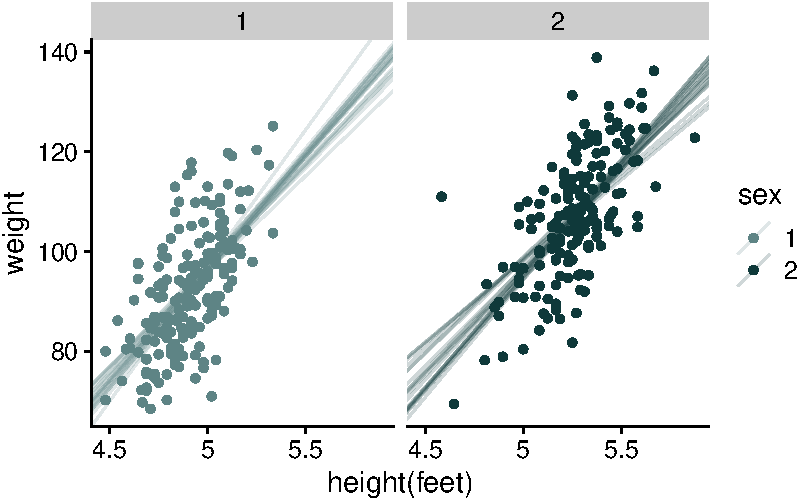
\includegraphics[width=17.1875in,height=\textheight]{lecture02-2_files/figure-pdf/unnamed-chunk-17-1.pdf}

\begin{center}\rule{0.5\linewidth}{0.5pt}\end{center}

\subsubsection{exercise}\label{exercise-2}

Return to the \texttt{milk} data. Write a mathematical model expressing
the energy of milk as a function of the species body mass
(\texttt{mass}) and clade category. Be sure to include priors. Fit your
model using \texttt{brms()}.

\begin{center}\rule{0.5\linewidth}{0.5pt}\end{center}

\subsubsection{solution}\label{solution-4}

\begin{align*}
K_i &\sim \text{Normal}(\mu_i, \sigma) \\
\mu_i &= \alpha_{\text{CLADE}[i]} + \beta_{\text{CLADE}[i]}(M-\bar{M})\\
\alpha_i &\sim \text{Normal}(0, 0.5) \text{ for }j=1..4 \\
\beta_i &\sim \text{Normal}(0, 0.5) \text{ for }j=1..4 \\
\sigma &\sim \text{Exponential}(1) \\
\end{align*}

\begin{Shaded}
\begin{Highlighting}[]
\NormalTok{milk}\SpecialCharTok{$}\NormalTok{mass\_c }\OtherTok{=}\NormalTok{ milk}\SpecialCharTok{$}\NormalTok{mass}\SpecialCharTok{{-}} \FunctionTok{mean}\NormalTok{(milk}\SpecialCharTok{$}\NormalTok{mass)}

\NormalTok{m4 }\OtherTok{\textless{}{-}} \FunctionTok{brm}\NormalTok{(}
  \AttributeTok{data =}\NormalTok{ milk,}
  \AttributeTok{family =}\NormalTok{ gaussian,}
  \FunctionTok{bf}\NormalTok{(K }\SpecialCharTok{\textasciitilde{}} \DecValTok{0} \SpecialCharTok{+}\NormalTok{ a }\SpecialCharTok{+}\NormalTok{ b}\SpecialCharTok{*}\NormalTok{mass\_c,}
\NormalTok{     a }\SpecialCharTok{\textasciitilde{}} \DecValTok{0} \SpecialCharTok{+}\NormalTok{ clade\_id,}
\NormalTok{     b }\SpecialCharTok{\textasciitilde{}} \DecValTok{0} \SpecialCharTok{+}\NormalTok{ clade\_id,}
     \AttributeTok{nl =} \ConstantTok{TRUE}\NormalTok{),}
  \AttributeTok{prior =} \FunctionTok{c}\NormalTok{(}\FunctionTok{prior}\NormalTok{( }\FunctionTok{normal}\NormalTok{(}\DecValTok{0}\NormalTok{,.}\DecValTok{5}\NormalTok{), }\AttributeTok{class=}\NormalTok{b, }\AttributeTok{nlpar =}\NormalTok{ a),}
            \FunctionTok{prior}\NormalTok{( }\FunctionTok{normal}\NormalTok{(}\DecValTok{0}\NormalTok{,.}\DecValTok{5}\NormalTok{), }\AttributeTok{class=}\NormalTok{b, }\AttributeTok{nlpar =}\NormalTok{ b),}
            \FunctionTok{prior}\NormalTok{( }\FunctionTok{exponential}\NormalTok{(}\DecValTok{1}\NormalTok{),  }\AttributeTok{class=}\NormalTok{sigma)),}
  \AttributeTok{iter =} \DecValTok{2000}\NormalTok{, }\AttributeTok{warmup =} \DecValTok{1000}\NormalTok{, }\AttributeTok{seed =} \DecValTok{3}\NormalTok{, }\AttributeTok{chains=}\DecValTok{1}\NormalTok{,}
  \AttributeTok{file =} \FunctionTok{here}\NormalTok{(}\StringTok{"files/models/22.4"}\NormalTok{)}
\NormalTok{)}
\end{Highlighting}
\end{Shaded}

\begin{center}\rule{0.5\linewidth}{0.5pt}\end{center}

\begin{Shaded}
\begin{Highlighting}[]
\FunctionTok{posterior\_summary}\NormalTok{(m4)}
\end{Highlighting}
\end{Shaded}

\begin{verbatim}
                  Estimate   Est.Error         Q2.5        Q97.5
b_a_clade_id1  -0.40476845 0.283412266  -0.94455375   0.16726235
b_a_clade_id2  -0.22553592 0.492279060  -1.17806955   0.74233613
b_a_clade_id3   0.34132362 0.432395484  -0.55499585   1.17621902
b_a_clade_id4  -0.01934509 0.507290802  -1.03169378   0.97077044
b_b_clade_id1  -0.00306615 0.008338136  -0.02027642   0.01268911
b_b_clade_id2  -0.05655136 0.042402253  -0.14149982   0.03104465
b_b_clade_id3  -0.04987753 0.054476898  -0.15271035   0.05688258
b_b_clade_id4   0.06473665 0.049274690  -0.03741264   0.15757431
sigma           0.79976985 0.119804429   0.59987239   1.06135351
lprior         -4.83595273 1.420149956  -8.20037391  -2.97899290
lp__          -39.39492980 2.284703218 -45.21163214 -36.02944463
\end{verbatim}

\begin{center}\rule{0.5\linewidth}{0.5pt}\end{center}

\begin{Shaded}
\begin{Highlighting}[]
\NormalTok{post }\OtherTok{=} \FunctionTok{as\_draws\_df}\NormalTok{(m4) }\SpecialCharTok{\%\textgreater{}\%} 
  \FunctionTok{pivot\_longer}\NormalTok{(}\FunctionTok{starts\_with}\NormalTok{(}\StringTok{"b"}\NormalTok{),}
               \AttributeTok{names\_to =} \FunctionTok{c}\NormalTok{(}\StringTok{"parameter"}\NormalTok{,}\StringTok{"clade\_id"}\NormalTok{),}
               \AttributeTok{names\_sep =} \DecValTok{3}\NormalTok{) }\SpecialCharTok{\%\textgreater{}\%} 
  \FunctionTok{mutate}\NormalTok{(}\AttributeTok{clade\_id =} \FunctionTok{str\_extract}\NormalTok{(clade\_id, }\StringTok{"[0{-}9]"}\NormalTok{)) }\SpecialCharTok{\%\textgreater{}\%} 
  \FunctionTok{pivot\_wider}\NormalTok{(}\AttributeTok{names\_from =}\NormalTok{ parameter, }\AttributeTok{values\_from =}\NormalTok{ value)}
\end{Highlighting}
\end{Shaded}

\begin{verbatim}
Warning: Dropping 'draws_df' class as required metadata was removed.
\end{verbatim}

\begin{Shaded}
\begin{Highlighting}[]
\NormalTok{milk }\SpecialCharTok{\%\textgreater{}\%} 
  \FunctionTok{ggplot}\NormalTok{(}\FunctionTok{aes}\NormalTok{(}\AttributeTok{x=}\NormalTok{mass\_c, }\AttributeTok{y=}\NormalTok{K)) }\SpecialCharTok{+}
  \FunctionTok{geom\_point}\NormalTok{(}\FunctionTok{aes}\NormalTok{(}\AttributeTok{color=}\NormalTok{clade\_id)) }\SpecialCharTok{+} 
  \FunctionTok{geom\_abline}\NormalTok{(}
    \FunctionTok{aes}\NormalTok{(}\AttributeTok{intercept=}\NormalTok{b\_a, }\AttributeTok{slope=}\NormalTok{b\_b, }\AttributeTok{color=}\NormalTok{clade\_id), }
    \AttributeTok{data=}\NormalTok{post[}\DecValTok{1}\SpecialCharTok{:}\DecValTok{80}\NormalTok{, ],}
    \AttributeTok{alpha=}\NormalTok{.}\DecValTok{2}
\NormalTok{  ) }\SpecialCharTok{+}
  \FunctionTok{facet\_wrap}\NormalTok{(}\SpecialCharTok{\textasciitilde{}}\NormalTok{clade\_id) }\SpecialCharTok{+}
  \FunctionTok{guides}\NormalTok{(}\AttributeTok{color=}\StringTok{"none"}\NormalTok{)}
\end{Highlighting}
\end{Shaded}

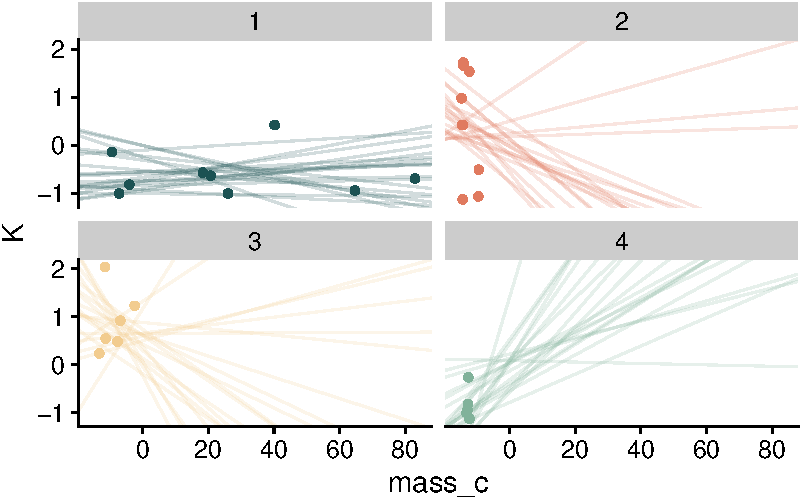
\includegraphics[width=17.1875in,height=\textheight]{lecture02-2_files/figure-pdf/unnamed-chunk-20-1.pdf}




\end{document}
